\documentclass[11pt, table, dvipsnames]{beamer}
%\documentclass[11pt,handout]{beamer}
\usepackage{xcolor}
\usepackage[all]{xy}

%\mode<beamer>{% 
%\usetheme[showothersubsections,right,width=17mm]{Goettingen}} 
%\usecolortheme{dove}
%\usecolortheme{lily}

%\mode<beamer>{\usetheme{Boadilla}}

\usepackage{hyperref}
 \title[Retrieving and Parsing Linguistic Expressions of Political Attitudes]{Retrieving Linguistic Expressions of Political Attitudes}
\author{Paul Nulty}
\institute % (optional)
{
  Department of Methodology, \\
  London School of Economics and Political Science, \\
  \vspace{2 mm}
  \textit{QUANTESS} ERC Project 
}
 
\date % (optional)
{Computational Social Science, ECCS 2014 \\ 
24th September 2014}


\graphicspath{ {./graphics/} }
\definecolor{customBlue}{rgb}{0.9,0.9,0.95}
\begin{document}

\begin{frame}%<handout:0>
\titlepage
\end{frame}


\begin{frame}
  \frametitle{Modes of information communication in online social networks}
 \begin{itemize}
  \item Network structure (friend, follower, subscriber)
  \item Simple actions: like, retweet, mention, favorite
  \item Multimedia: links, animations, videos, images
  \item Linguistic (text): Posts, comments, tweets
  \end{itemize}
\end{frame}

\begin{frame}
  \frametitle{Introduction}
  \begin{itemize}
  \item Text is a hugely rich but unstructured information source
  \item Social media offers large, real-time corpus of spontaneous communication and expression
  \item Retrieval depends on bursty and ambiguous search terms
  \item Simple word frequency matrix methods, also rich latent structure
  \item NLP offers methods to discover structure and help retrieval
  \item Twitter`s communication model makes it especially useful
  \end{itemize}
\end{frame}

\begin{frame}
  \frametitle{Natural language on twitter}
  \begin{itemize}
  \item Text is the principal mode of communication broadcast on twitter
  \item Limit on post length causes some issues, but fixable \footnote{Syntactic normalization of twitter messages, Kaufman and Kalita 2010)}
  \item Simple statistical linguistics can aid retrieval
  \item Linguistic structure can be identified with parsing
  \end{itemize}
\end{frame}

\begin{frame}
  \frametitle{Zipf's laws}
  \begin{itemize}
  \item In natural languages, word frequencies have a very heavy-tailed distribution
  \item Zipf's Law (1935): The frequency of a word is inversely proportional to its rank in the frequency table
  \item Zipf (1945): The more frequent a word is, the more senses it is likely to have
  \item frequent search terms give high recall, but low precision
  \end{itemize}
\end{frame}




\begin{frame}
  \frametitle{Rank frequency of terms}

    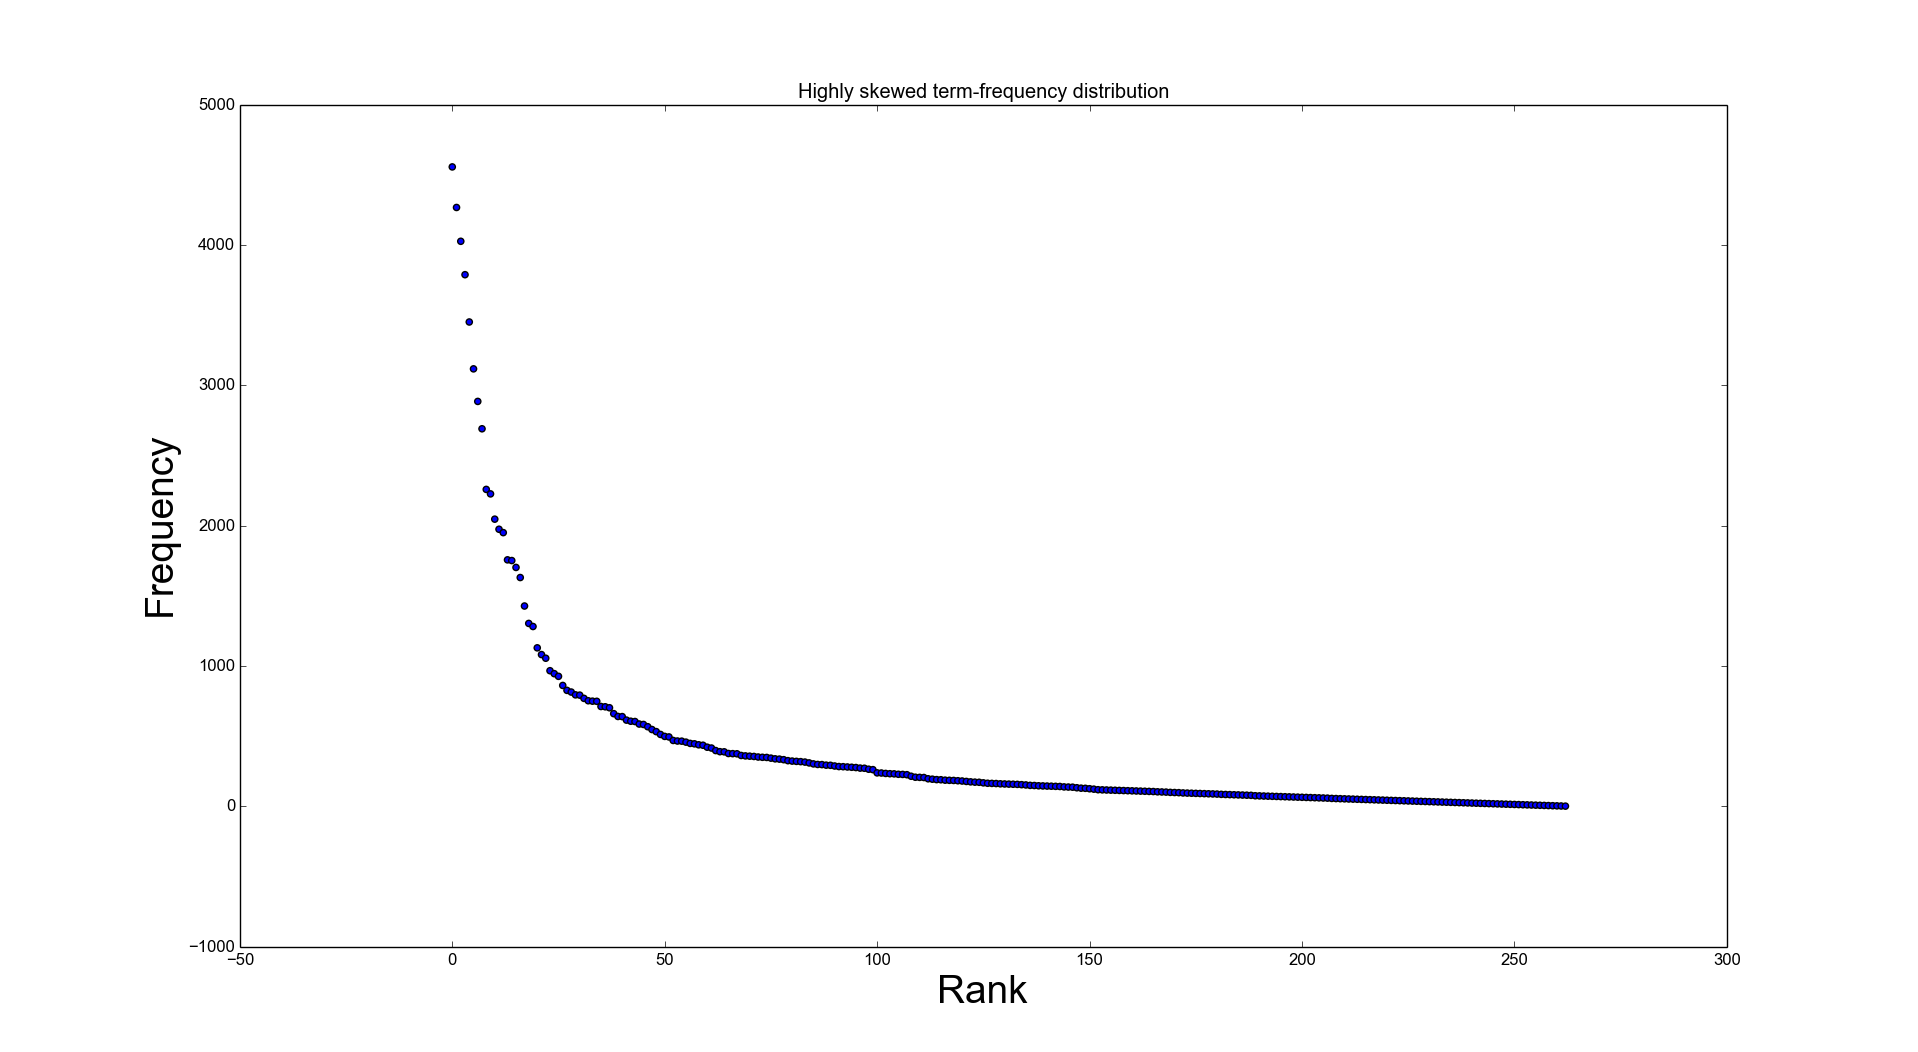
\includegraphics[scale=0.20]{zipf1}
  \scriptsize
  Data from 260,619 tweets (no retweets), from twitter `gardenhose' api on Scottish referendum day, containing any of these terms: \texttt{["\#indyref", "salmond", "cameron", "scotland", "scottish", "referendum", "vote", "voted", "voting"]}
\end{frame}

\begin{frame}
  \frametitle{Log-Log Rank frequency}

    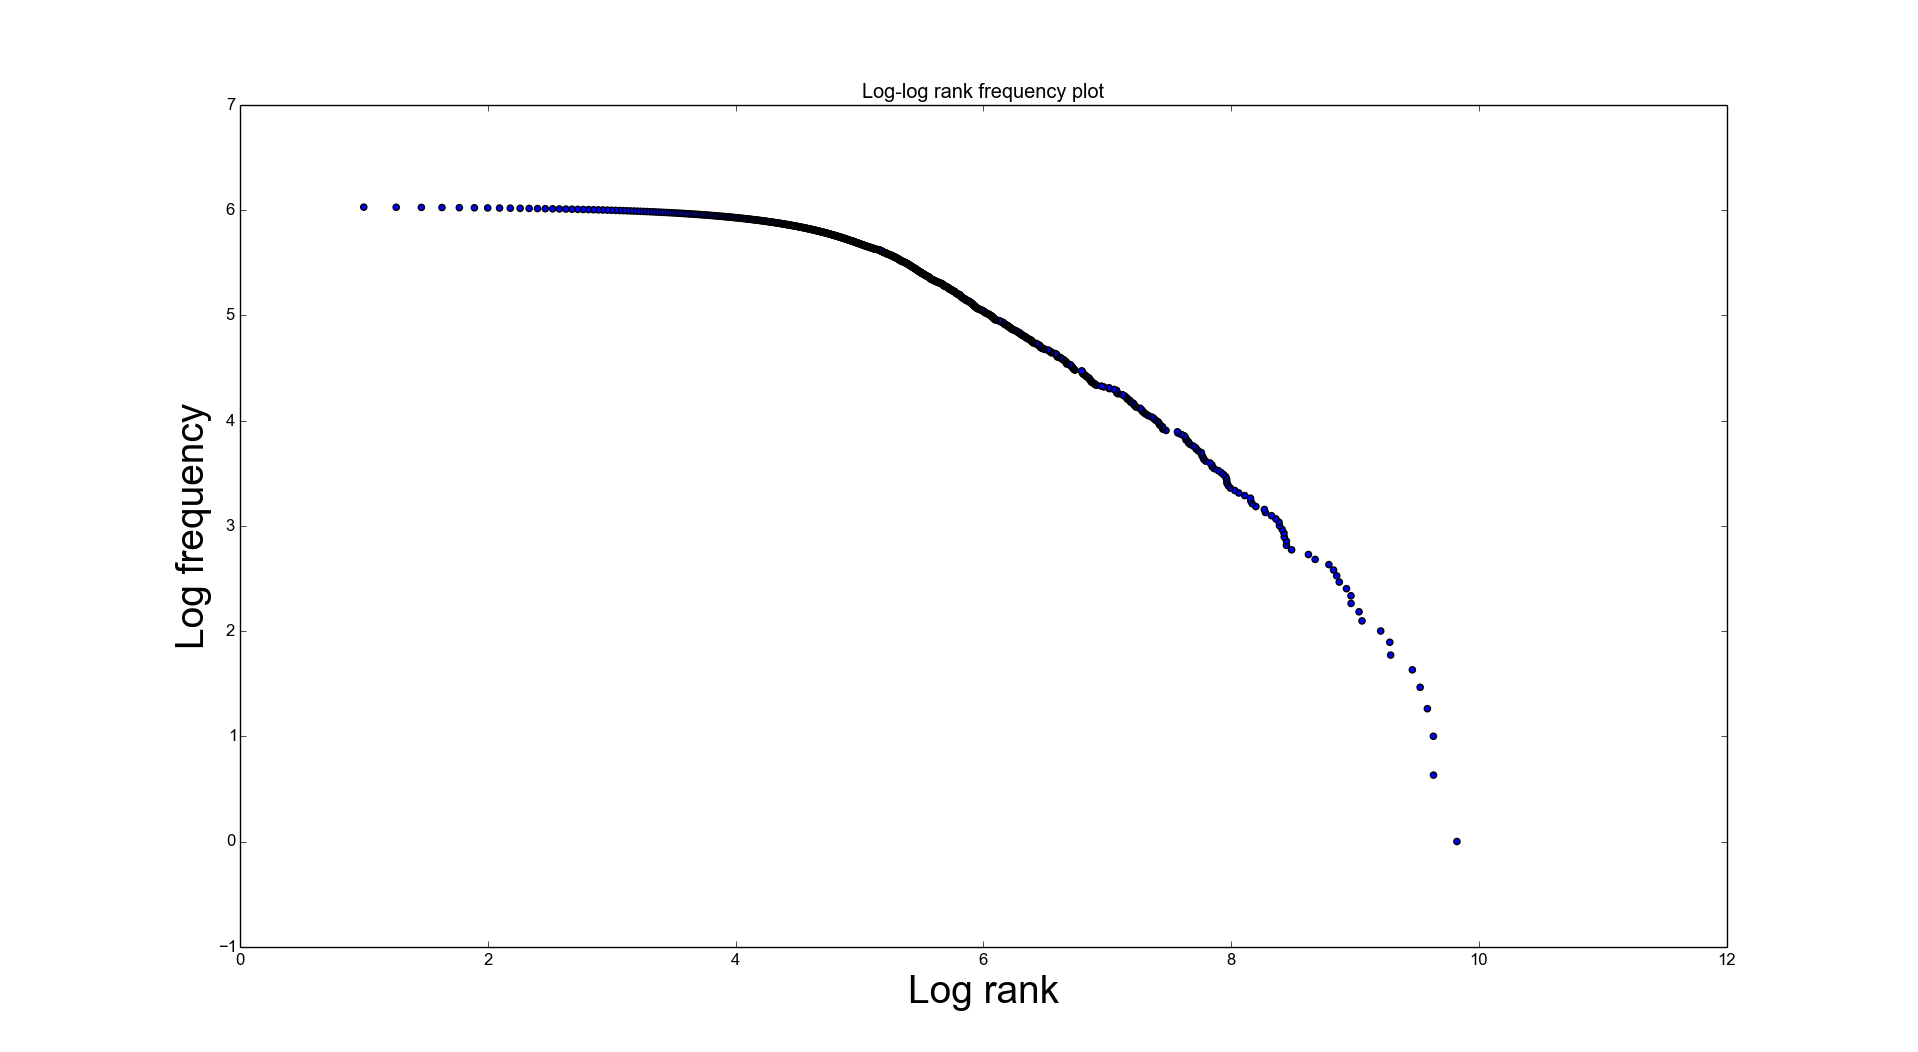
\includegraphics[scale=0.20]{zipf2}
  \scriptsize
  Data from 260,619 tweets (excluding retweets, 1.02M total), from twitter `gardenhose' api on Scottish referendum day, containing any of these terms: \texttt{["\#indyref", "salmond", "cameron", "scotland", "scottish", "referendum", "vote", "voted", "voting"]}
\end{frame}

\begin{frame}
  \frametitle{Discovering query terms with a classifier}
  \begin{itemize}
  \item Initially, prefer recall over precision
  \item Hone search terms by learning association between terms and concept of interest
  \item e.g. Initially search for "vote", "cameron", "indyref"
  \item learn which terms co-occur with precise terms of interest
  \end{itemize}
\end{frame}

\begin{frame}
  \frametitle{Example Naive Bayes classifier}
  \begin{itemize}
  \item Train 
  \item Simple bag-of-words model
  \item 
  \end{itemize}
\end{frame}

\begin{frame}
\frametitle{terms predictive of 'no'(bettertogether and nothanks}
  \begin{table}[!htbp]\centering
  \rowcolors{1}{customBlue}{White}
\begin{tabular}{p{4cm}p{3.5cm}p{1.5cm}}
 \hline
term & Direction & Ratio \\
\hline
kingdom        &         no   &    20.7 \: 1.0 \\
stupid         &       no    &     16.1 \: 1.0 \\
united          &       no    &     15.0 \: 1.0 \\
stay           &     no    &      8.9 \: 1.0 \\
\hline
\end{tabular}
\end{table}
\end{frame}
%
%
%         \#freedom = 1.0               yes : no     =     29.8 : 1.0
%      \#letsdothis = 1.0               yes : no     =     20.9 : 1.0
%                 
%         \#voteaye = 1.0               yes : no     =     20.2 : 1.0
%           \#savvy = 1.0               yes : no     =     18.0 : 1.0
%        
%                 imagine = 1.0               yes : no     =      9.8 : 1.0
%             opportunity = 1.0               yes : no     =      9.4 : 1.0
%                  fairer = 1.0               yes : no     =      9.2 : 1.0
%                    stay = 1.0                no : yes    =      8.9 : 1.0
%              \#no = 1.0                no : yes    =      8.6 : 1.0
%    \#hopeoverfear = 1.0               yes : no     =      8.1 : 1.0
%                   hands = 1.0               yes : no     =      7.6 : 1.0
%                 society = 1.0               yes : no     =      7.0 : 1.0
%    \#independence = 1.0               yes : no     =      6.7 : 1.0
%              \#uk = 1.0                no : yes    =      6.6 : 1.0
%                 excited = 1.0               yes : no     =      6.3 : 1.0
%  \#votenoscotland = 1.0                no : yes    =      6.1 : 1.0
%    atsymbnicolasturgeon = 1.0               yes : no     =      5.9 : 1.0
%                   brave = 1.0               yes : no     =      5.5 : 1.0
%          \#voteno = 1.0                no : yes    =      5.5 : 1.0
%                   youve = 1.0               yes : no     =      5.3 : 1.0
%                   union = 1.0                no : yes    =      5.2 : 1.0
%                    18th = 1.0               yes : no     =      5.0 : 1.0
%                    fear = 1.0               yes : no     =      5.0 : 1.0
%                  enough = 1.0                no : yes    =      4.8 : 1.0
%                  chance = 1.0               yes : no     =      4.8 : 1.0
%                   sense = 1.0                no : yes    =      4.8 : 1.0
%  \#bettertogether = 0.0               yes : no     =      4.7 : 1.0
%                     aye = 1.0               yes : no     =      4.6 : 1.0
%                      uk = 1.0                no : yes    =      4.4 : 1.0
%                    cmon = 1.0               yes : no     =      4.4 : 1.0
%                 britain = 1.0                no : yes    =      4.3 : 1.0
%                   leave = 1.0                no : yes    =      4.3 : 1.0
%                yourself = 1.0               yes : no     =      4.2 : 1.0
%                  hoping = 1.0                no : yes    =      4.2 : 1.0
%                    felt = 1.0               yes : no     =      4.1 : 1.0
%               emotional = 1.0               yes : no     =      4.1 : 1.0
%                 control = 1.0               yes : no     =      4.1 : 1.0
%                  anyone = 1.0                no : yes    =      4.0 : 1.0
%                together = 1.0                no : yes    =      3.9 : 1.0

\begin{frame}
\frametitle{out of sample prediction of \#bettertogether v \#voteyes}
  \begin{itemize}
  \item 800 most common terms
  \item removed labelled terms
  \item predicted 2028 \/ 2630 correctly (77\%)
  \end{itemize}
\end{frame}




\end{document}
